
\subsection{Zero to the zero power}
The following example draws a graph of the function $f(x)=|x^x|$.
The graph shows why the convention $0^0=1$ makes sense.

\begin{Verbatim}[formatcom=\color{blue},samepage=true]
f(x) = abs(x^x)
xrange = (-2,2)
yrange = (-2,2)
draw(f,x)
\end{Verbatim}

\begin{center}
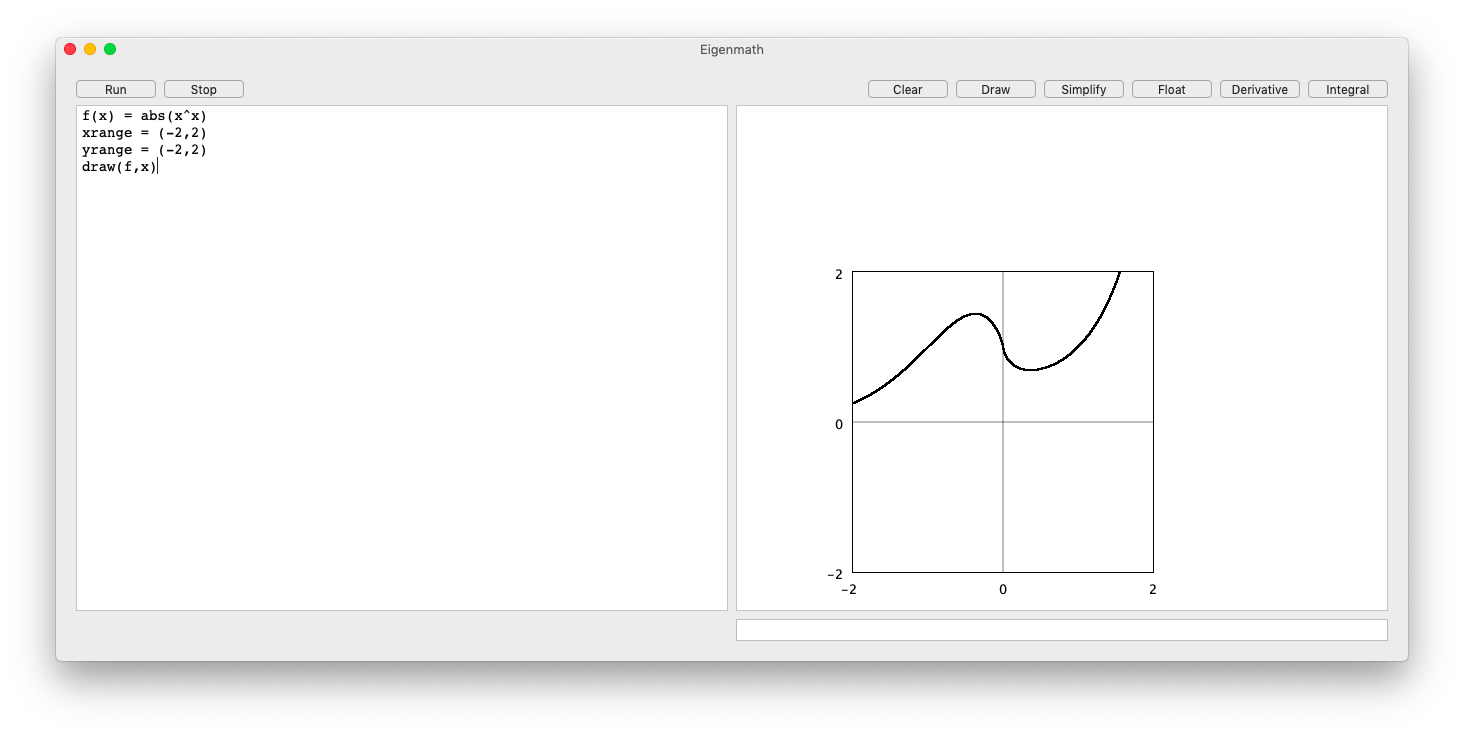
\includegraphics[scale=0.2]{zerozero.png}
\end{center}

We can see how $0^0=1$ results in a continuous line through $x=0$.
Now let us see how $x^x$ behaves in the complex plane.

\begin{Verbatim}[formatcom=\color{blue},samepage=true]
f(t) = (real(t^t),imag(t^t))
xrange = (-2,2)
yrange = (-2,2)
trange = (-4,2)
draw(f,t)
\end{Verbatim}

\begin{center}
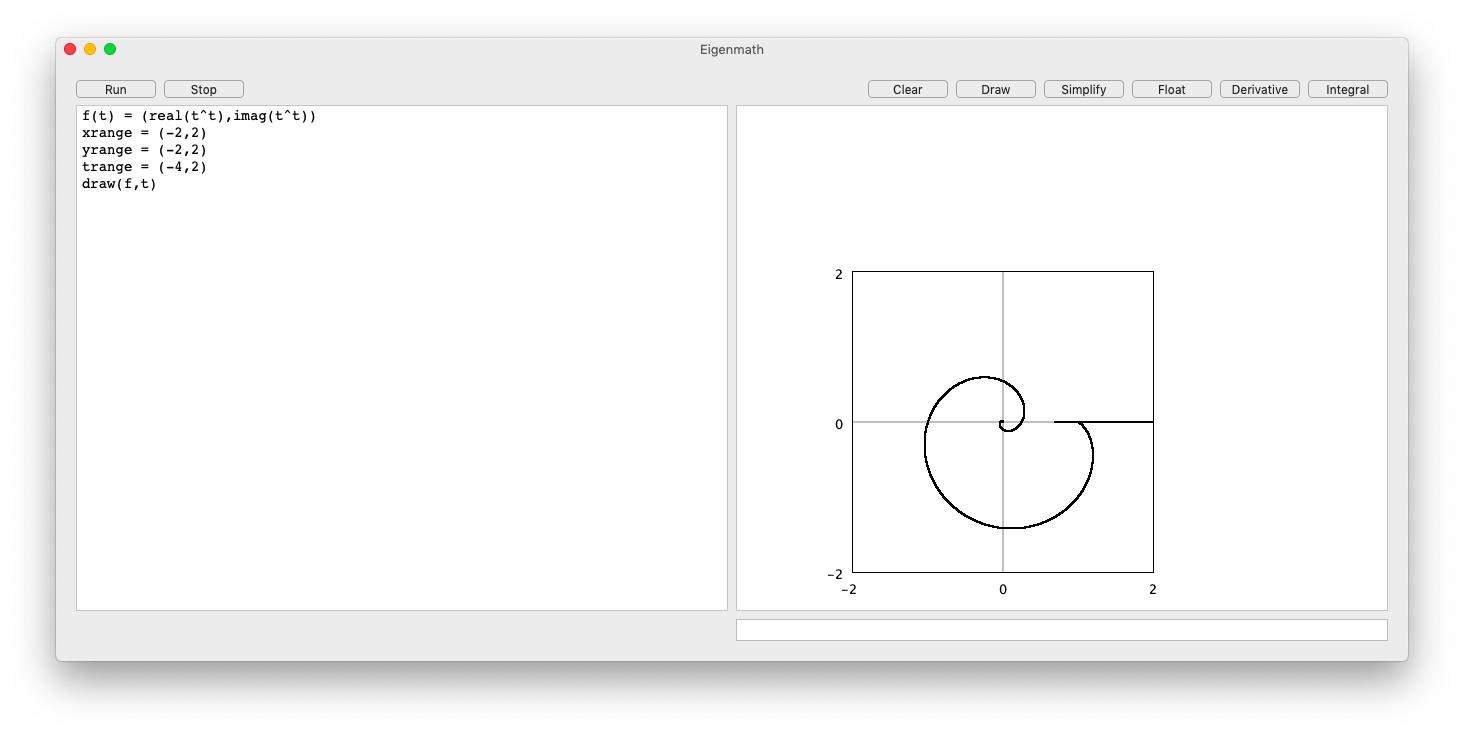
\includegraphics[scale=0.2]{zerozero2.png}
\end{center}
